\clearpage
\section{Cow Protocol}

\begin{refsection}

\begin{tcolorbox}	
\begin{tabular}{p{2.75cm} p{0.2cm} p{10.5cm}} 	
\textbf{Student Name}  &:&  Jo\~ao Ant\'onio\\
\textbf{}  & &  Daniel Pereira\\
\textbf{Goal}          &:& Explain the Coherent One Way (COW) Protocol and test it's strength against a intercept resend attack.\\
\textbf{Directory}     &:& sdf/tq\_76558\_cow\_protocol
\end{tabular}
\end{tcolorbox}

A Quantum Key Distribution (QKD) is a secure way of communicating between two parties spatially distant using properties of quantum mechanics. This connection creates random key with ones and zeros, by doing a sum (mod 2), between the key and the message, we can encrypt a message, if we later use, again a sum (mod 2) in the encrypted message, we decrypt it, obtaining the original message allowing the person to read it. This is how the One Time Pad (OTP) works, that was patented by Vernam and well tested, for example, \cite{glover2005one}. This OTP is one of the protocols that can be used to encrypt and decrypt messages, where both users have the same key, the QKD is the protocol responsible to make sure that both parties (Alice and Bob, as they are usually called) have the same key, and that it is secure.

The importance of the "Quantum" in QKD arouses from the fact that the classic ways of creating and sharing the random secret key are quickly becoming unreliable, mostly due to the work in quantum computers.

The QKD protocols can use either discrete variables or continuous variables, and the ones that use discrete variables can use either polarization or time bin encoding \cite{singh}. The most well know QKD is the BB84 that uses discrete variables and polarization to codify information \cite{bennett1992quantum}.

\begin{figure}[h]
\centering
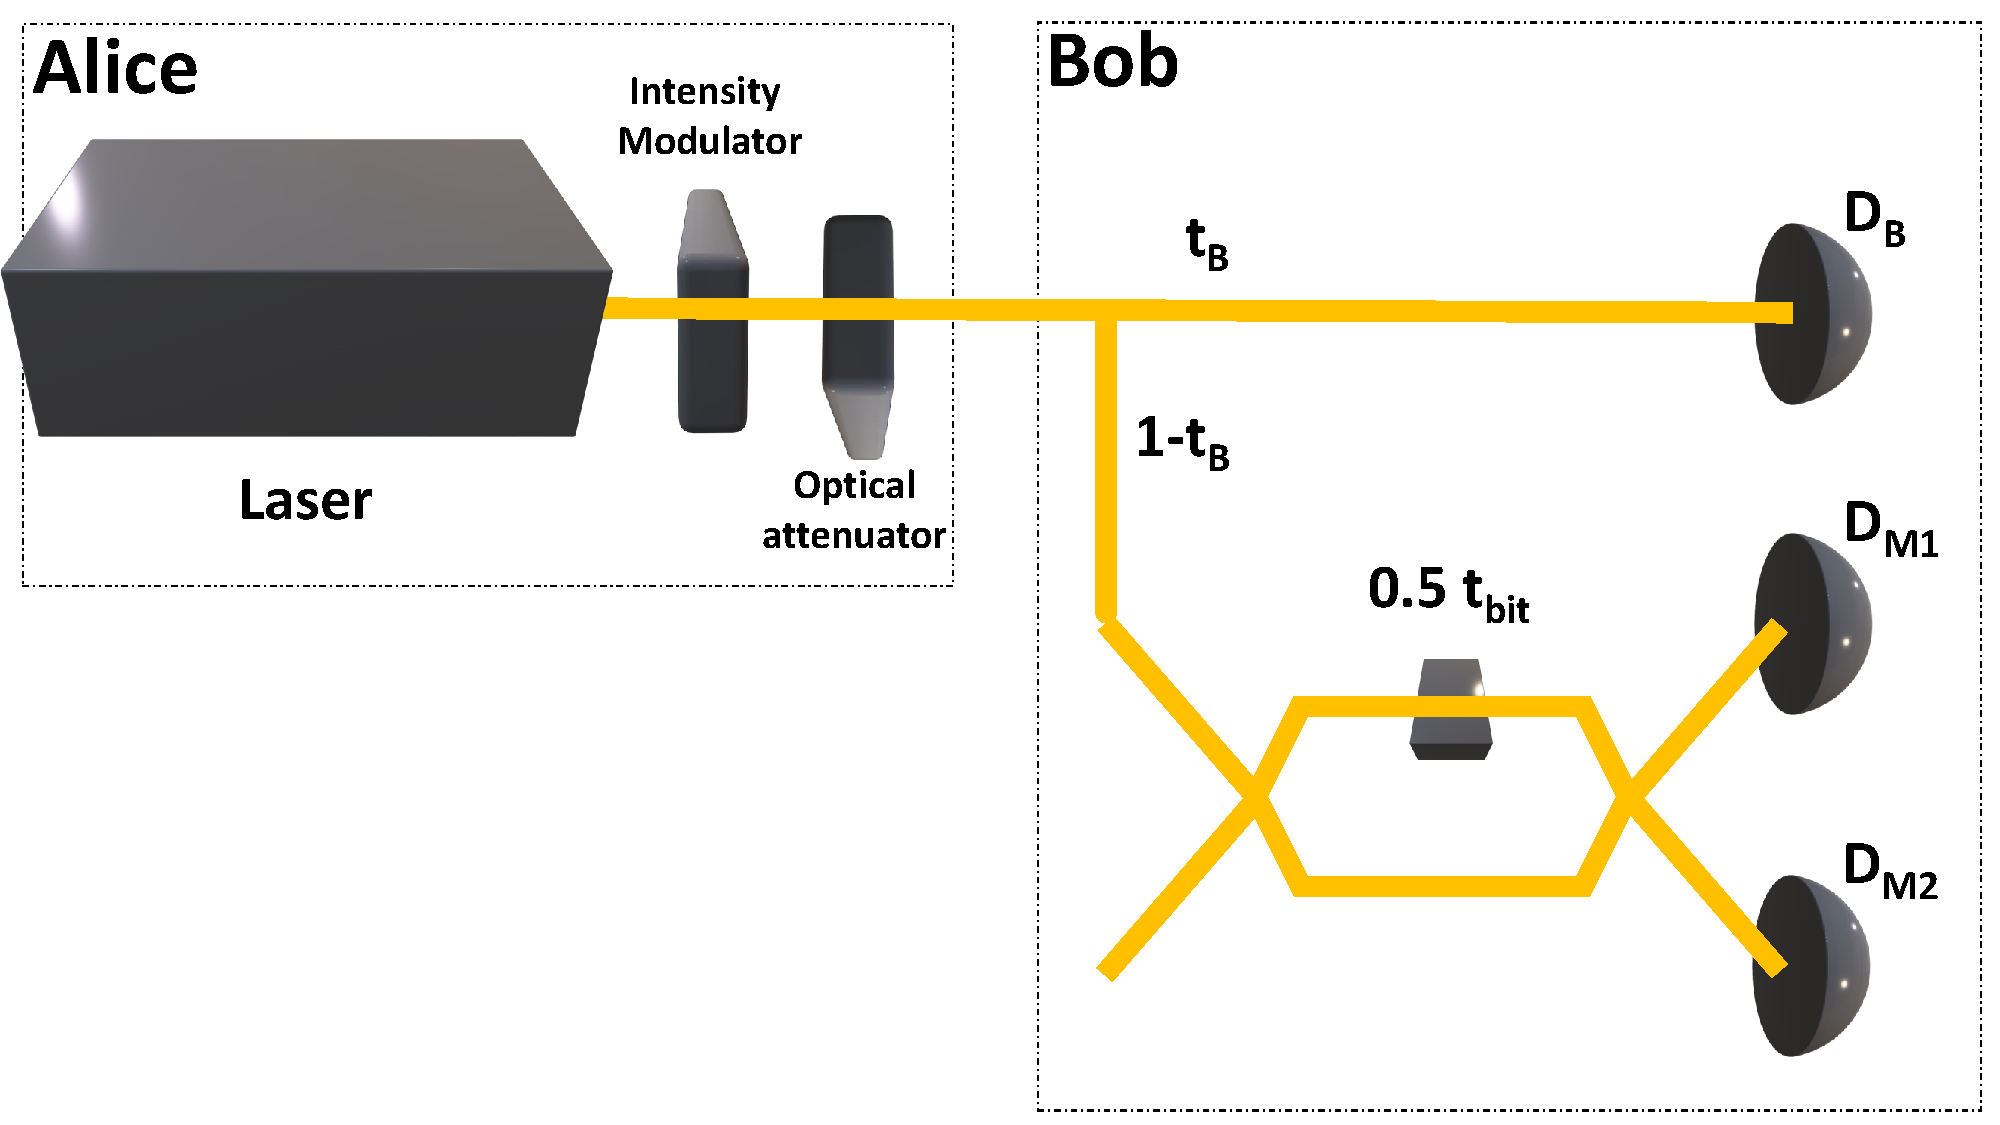
\includegraphics[width=1\linewidth]{./sdf/tq_76558_cow_protocol/slides/figures/Full2.pdf}
\caption{Simple scheme of the COW protocol.}
\label{fig:Scheme}
\end{figure}

The Coherent One Way (COW) protocol is another QKD protocol that also uses discrete variables but uses time bin encoding, meaning that the information is passed in the time bins and not in the polarization like the BB84.

The COW protocol was created by Nicolas Gisin et al in 2004 in \cite{gisin2004towards}, and as a very simple set-up, it was already very well tested against various attacks like \cite{branciard2006zero}, tested with some real prototypes \cite{stucki2009continuous} and it is already being commercialized by companies like ID Quantic. A simple scheme of the COW protocol can be seen in the Figure \ref{fig:Scheme} (it is worth noting that a few modifications experimental set up was already proposed \cite{roberts2017modulator} to reduce cost and sometimes to increase the quantity of information by second, not altering in anything the protocol, I remained with the most common, the original)

In this article I explore the Cow protocol and do a simulation of a basic intercept-resend attack. In the quantum cryptography world is common to do attacks on the protocol to test their security, this attack is one of the simplest one where Eve (an eavesdropping) collects all the information and sends it to the Bob.

\subsection{Theoretical Analysis}

This protocol as the name implies (Coherent One Way) uses a one-directional quantum channel and an authenticated classic channel, authenticated meaning that can be eavesdropped but can't be modified.

In the first step of the protocol, Alice creates a random key using and forwards it through the quantum channel to Bob, the notation used here is the same on the \cite{gisin2004towards} and to help visualize I have created Fig. \ref{fig:sta}.

$$|0\rangle = |\alpha\rangle_{2K-1} |\emptyset\rangle_{2K} =\ \ Logical\ 0\ $$

$$|1\rangle = |\emptyset\rangle_{2K-1} |\alpha\rangle_{2K} =\ \ Logical\ 1\ $$

$$|d\rangle = |\alpha\rangle_{2K-1} |\alpha\rangle_{2K} = Decoy State$$

Where $|\emptyset\rangle$ is the vacuum state and $|\alpha\rangle$ is a coherent state of light with intensity $\mu=|\alpha|^2<<1$.
The probability of creating a $|0\rangle$ state and a $|1\rangle$ is equal, the probability of creating a $|d\rangle$ state is usually 10 \%.

\begin{figure}[hbt!]
\centering
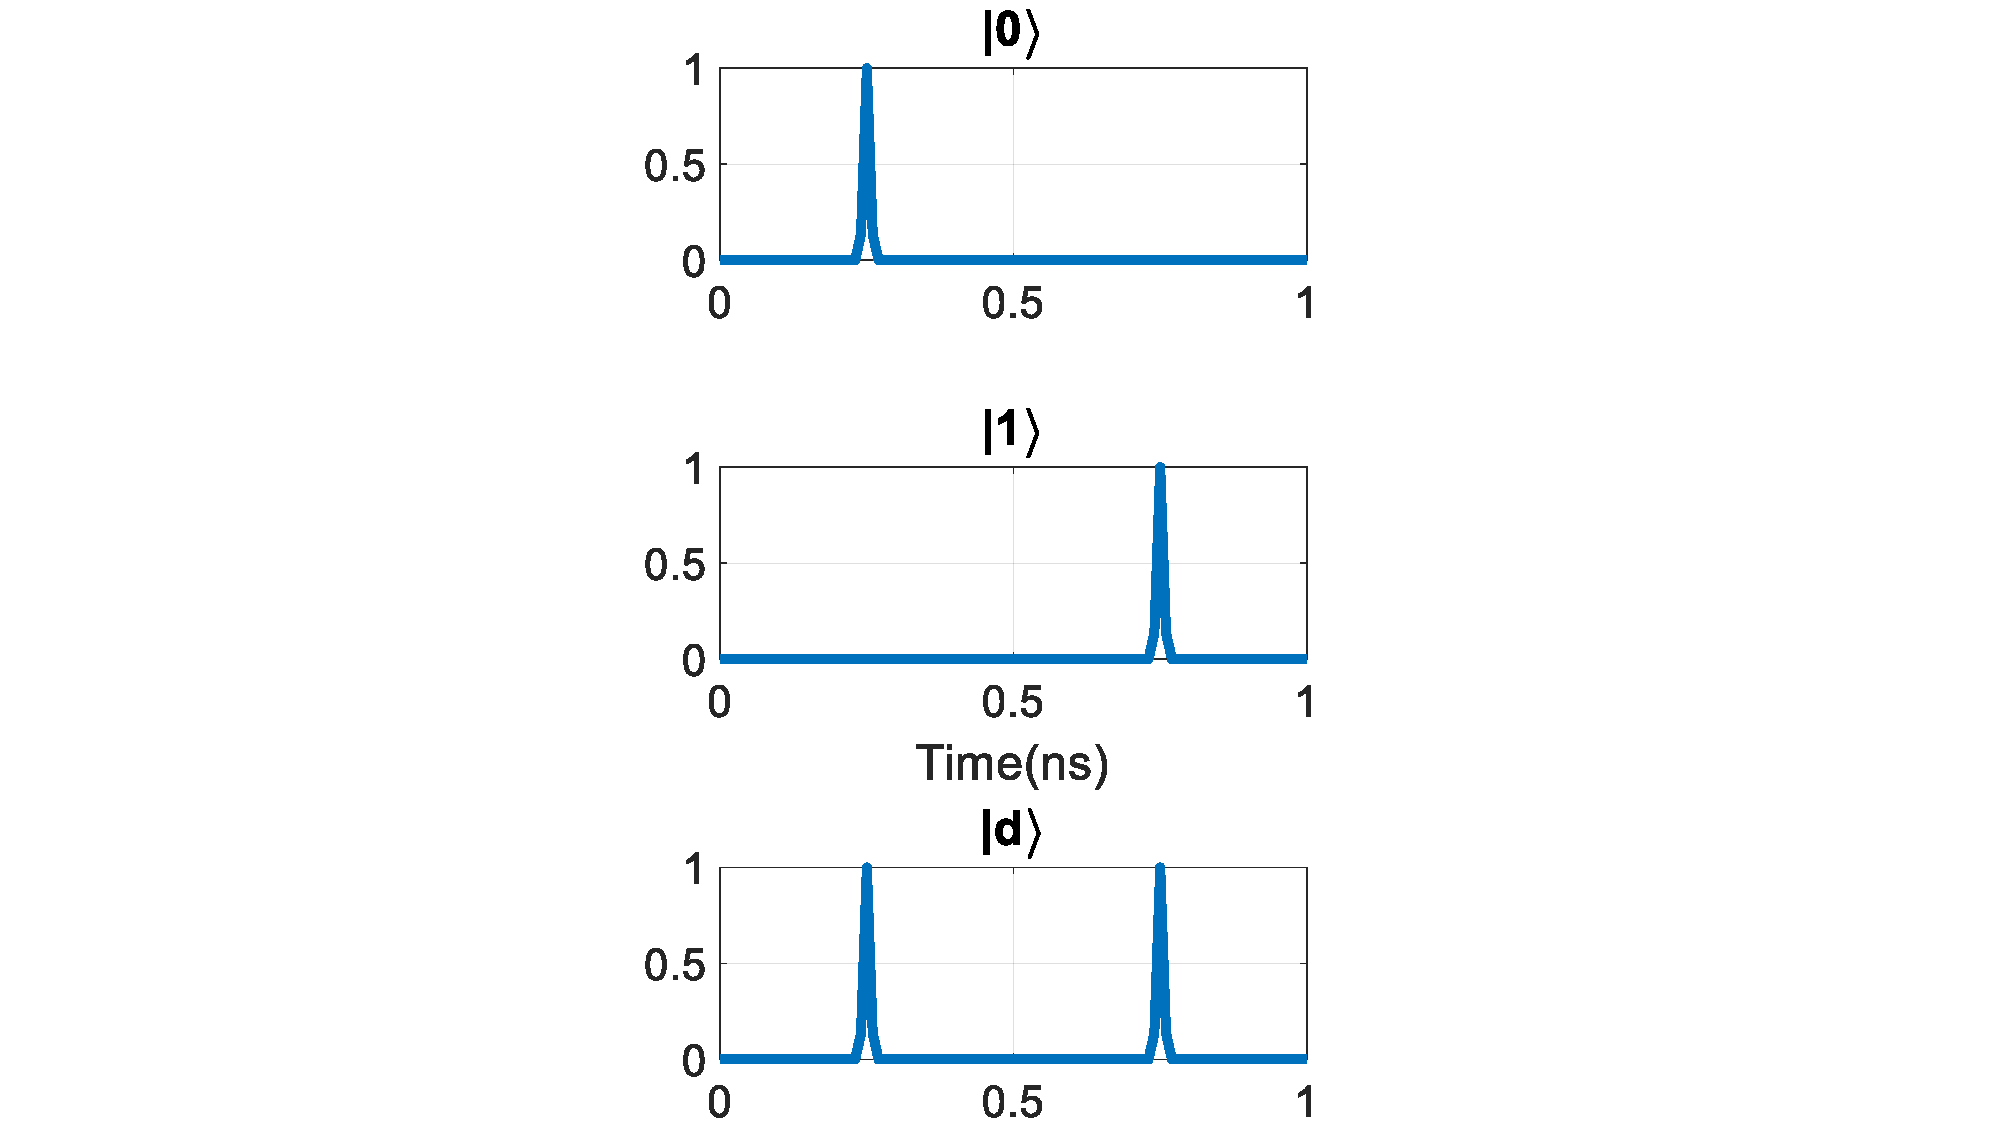
\includegraphics[width=1\linewidth]{./sdf/tq_76558_cow_protocol/slides/figures/S1A.pdf}
\caption{Representation of the possible states.}
\label{fig:sta}
\end{figure}

The average number of photons by impulse is modulated by a Poisson distribution with $\lambda=0.1$. With this is mind the probability of a decoy state having both the peaks with at least one photon each is 1\%. If instead we used a bigger average number of photons by impulse, it would make the protocol hazardous against the most basic kind of attacks, beam splitter attacks, where Eve would remove a portion of photons by impulse and Bob and Alice wouldn't even notice \cite{kronberg2017analysis}.

On the second step, Bob receives the photons in his apparatus. Here a fraction $t_B$ of the photons go into the photon counter $D_B$ (data line), where the bits are discriminated by the time of arrival, while the rest of the photons go to the monitoring line. This fraction $t_B$ is usually 90\%, so 90\% of the photons go to the data line and are used to create the key, the other 10\% of photons go to the monitoring line and are used to test the security of the communication.

Bob has three photons detectors in his apparatus, in \cite{gisin2004towards} they use 10\% efficiency and a probability of dark count of $10^-5$ for all photon detectors. A dark count is what happens when the detector falsely fires.Meaning that if an impulse as ten photons, in average, nine go to the data line and one goes in to the monitoring line. If the impulse as one photon 90\% of the time it goes to the data line and 10\% it goes to the monitoring line. In this monitoring line, the photons have a 50 \% probability of being delayed by 0.5 $t_{bit}$ and 50\% of not being delayed. 

If a photon that arrived at the monitoring line in $time=0$ is delayed to the $time=0.5$, and one photon on the $time=0.5$ is not delayed they will interact. When this happen the $D_{M2}$ (constructive photon counter) will try to click (not guaranteed due only to the efficiency of the detector). Based on this we know that are only two cases in which the $D_{M2}$ can click, or in a $|d\rangle$ state or in the $|1\rangle$ state followed by the $|0\rangle$ state, to having the $D_{M2}$ click we know that at least two impulses were consecutive, I represented this in Fig.\ref{fig:dm2}.

\begin{figure}[hbt!]
\centering
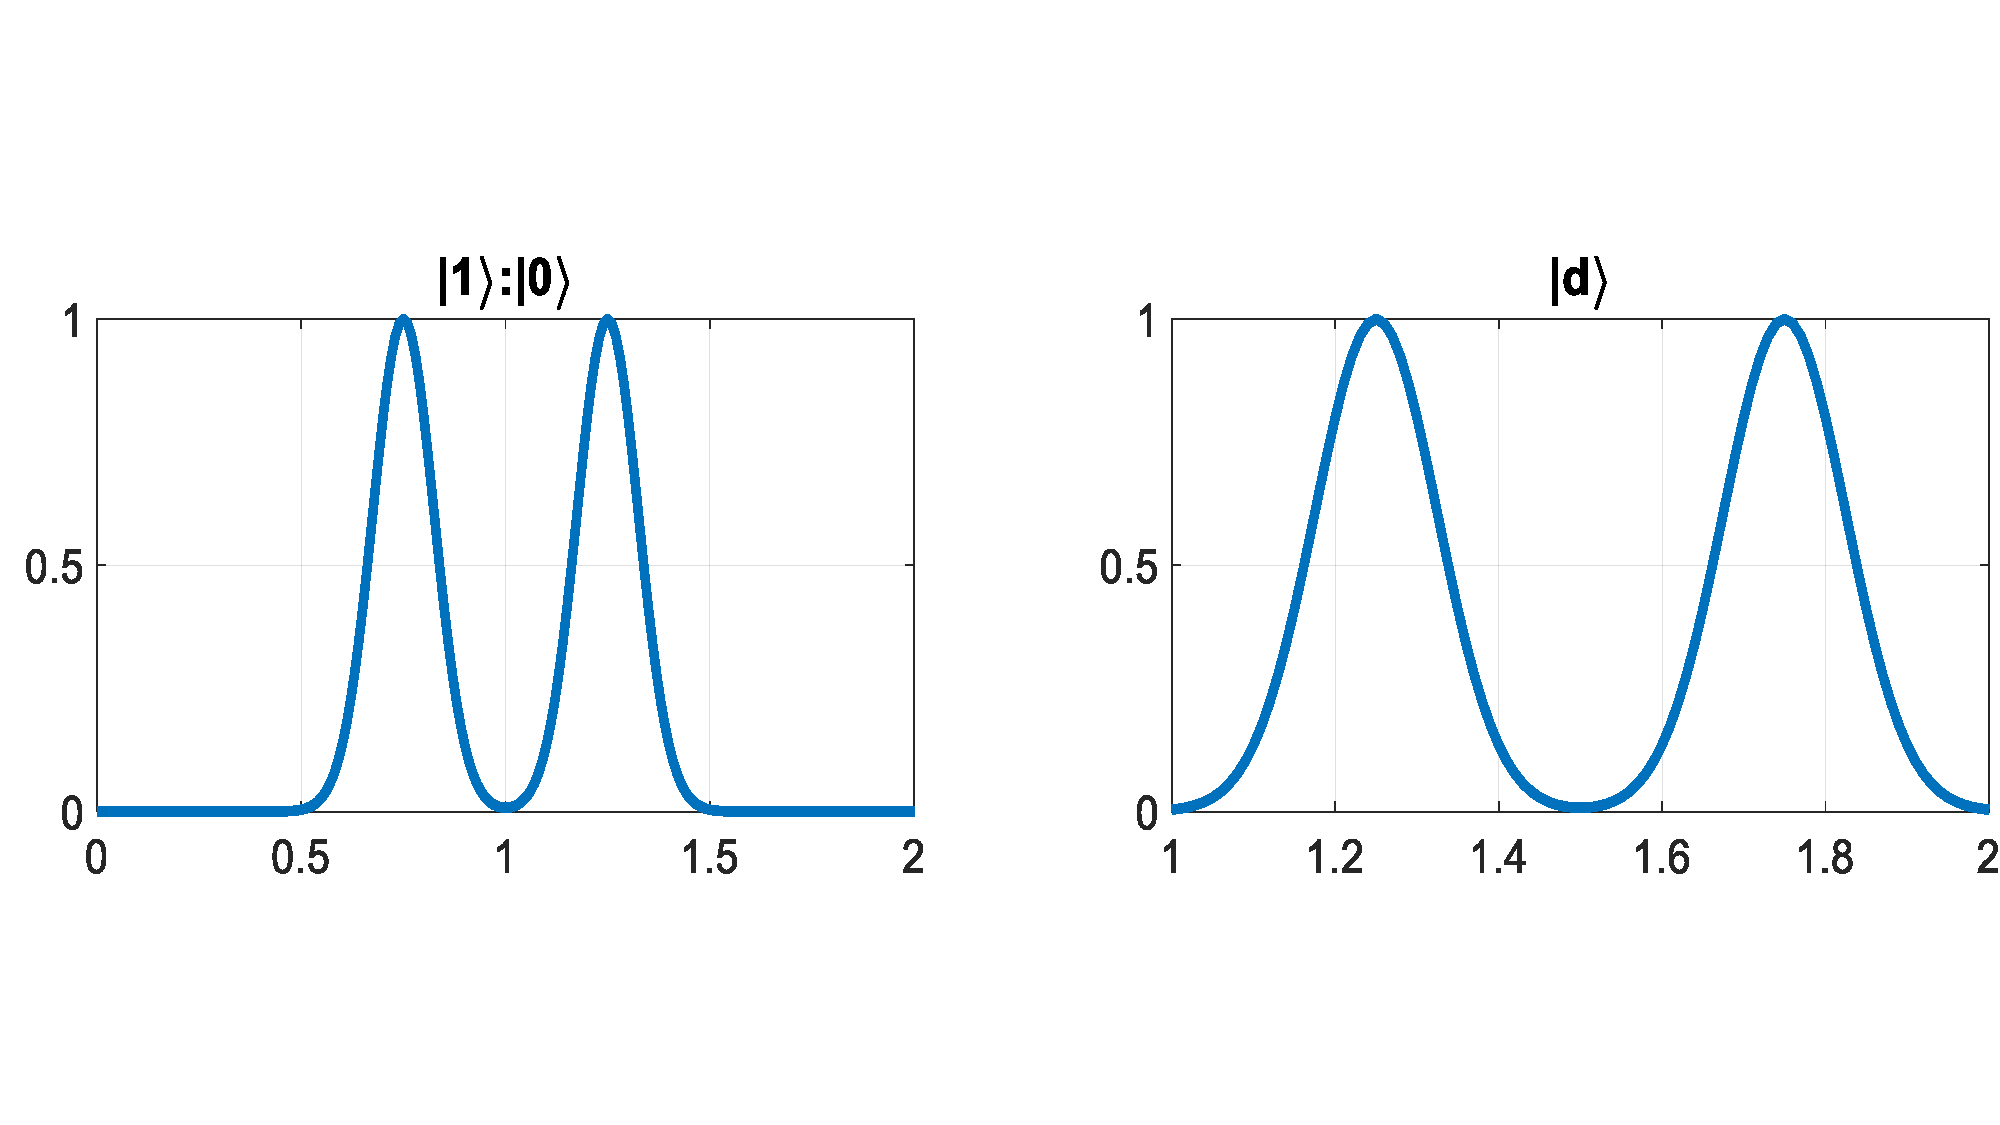
\includegraphics[width=1\linewidth]{./sdf/tq_76558_cow_protocol/slides/figures/S2.pdf}
\caption{Events where the $D_{M2}$ (constructive photon counter) clicks.}
\label{fig:dm2}
\end{figure}

Note that if the impulses are generated by different lasers, they will not be coherent, so the $D_{M2}$ will not click, to click the two impulses need to be consecutive and coherent (generated by the same laser) \cite{rusca2018security}.

In all the other cases were two photons don't interact, the $D_{M1}$ clicks (or tries to, due to the efficiency), meaning that if the impulse of $|1\rangle$ followed by another impulse $|1\rangle$ go into the monitoring line, the $D_{M1}$ will click twice (assuming 100\% efficiency), because they can't interact with each other, the impulses are distanced by 1 $t_{bit}$. In another example, analysing the Fig.\ref{fig:dm3}, in this Figure we have at blue the raw key that enters the monitoring line, supposing that all impulses have multiple photons, we have the $D_M2$ clicking six times just like is represented in the figure, if we assume that all impulses only have one photon we can have the $D_{M2}$ clicking between zero and five times. Zero times if all the photons that get to the monitoring line are delayed, they will never interact among them so the $D_{M2}$ will never click. Five times as the maximum if they are all single photons, because if they are all single photons the $D_{M2}$ will never click two times consecutively ($times=8.5$ and $9$), because a photon can't be delayed and not delayed at the same time interacting with both other photons.

But resuming conditions of the image (efficiency of 100\%, 0\% probability of dark count, multiples photons by impulse), we can see that all the situations where we have impulses or delayed impulses and the $D_{M2}$ hasn't clicked the $D_{M1}$ clicks. It's other noting that are times (like $time=6$ or $time=0$) that none of the detectors clicks.

\begin{figure}[hbt!]
\centering
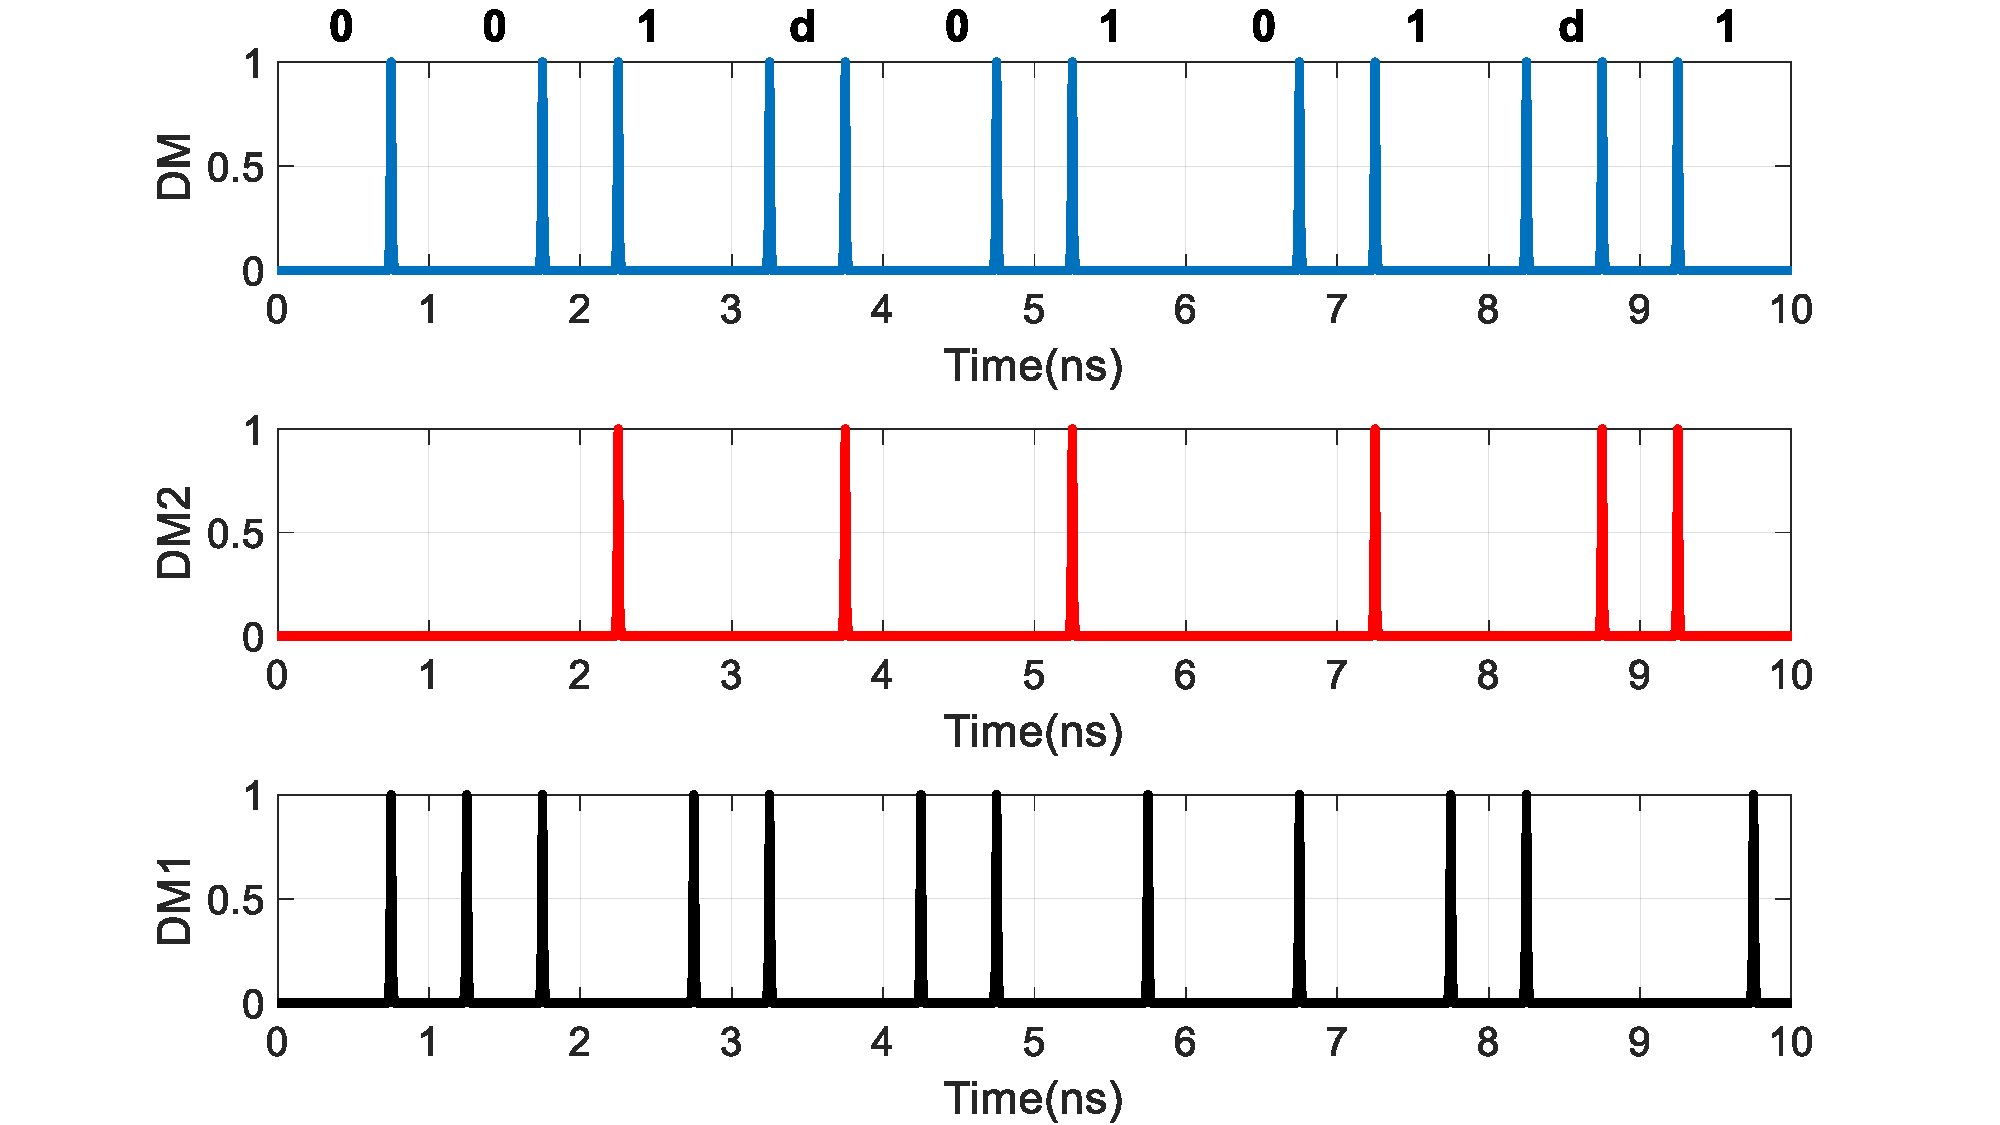
\includegraphics[width=1\textwidth]{./sdf/tq_76558_cow_protocol/slides/figures/DM3.pdf}
\caption{Random key and the DM1 and DM2 clicks}
\label{fig:dm3}
\end{figure}

For the next step (3), Alice tells Bob the decoy times, he removes this times from the data Line, example cases where only the first impulse of the decoy state had a photon, Bob detected it as $|0\rangle$ and Alice had sent a decoy, so the key would have more errors if he didn't remove this from the data. Bob also checks if some of the times that the $D_{M2}$ clicked belong to the decoys.

After he tells Alice all the other times that the $D_{M2}$ clicked, Alice checks that they belong to $|0\rangle$ followed by $|1\rangle$ states. I have called this step the forth. If they don't belong to this state (Bob has already removed the decoy states) means that someone introduced more impulses that the ones that she sent. If the $D_{M2}$ has clicked much lesser times than expected means that there is someone in the line that in generating the pulses in various lasers, breaking the coherence, reducing the $D_{M2}$ counts.

Afterwards, in step five, Bob reveals the times that he had a detection in the data line, this allows Alice to remove from her key all the times were the photon was absorbed by the fibber, or the impulse was to the monitoring line.

Finally (in the sixth step) they calculate QBER and compare the values of detection that they obtained with the ones that are predicted by theory and statics, if those two properties are okay, they proceed to the next step that consist in run error correction and privacy amplification. In the end of this seventh step they have the final key.

\subsection{Simulation Analysis}

With the protocol explained, I wanted to test his security, the most basic attack like a beam splitter has said previously due to the average number of photons by impulse was doomed to fail completely, one of the next attacks to consider is a basic intercept resend attack (IR). On this attack Eve captures all the information, measures and then resend it to Bob, it is considered a basic attack because she does this during all the communication, a more advance IR attack would be turned on and off to make it more difficult to be detected. For representing the system used I have created a block diagram in Fig.\ref{fig:bloc} and a representation using the same blocks as previously in Fig.\ref{fig:E}.

\begin{figure}[h]
\centering
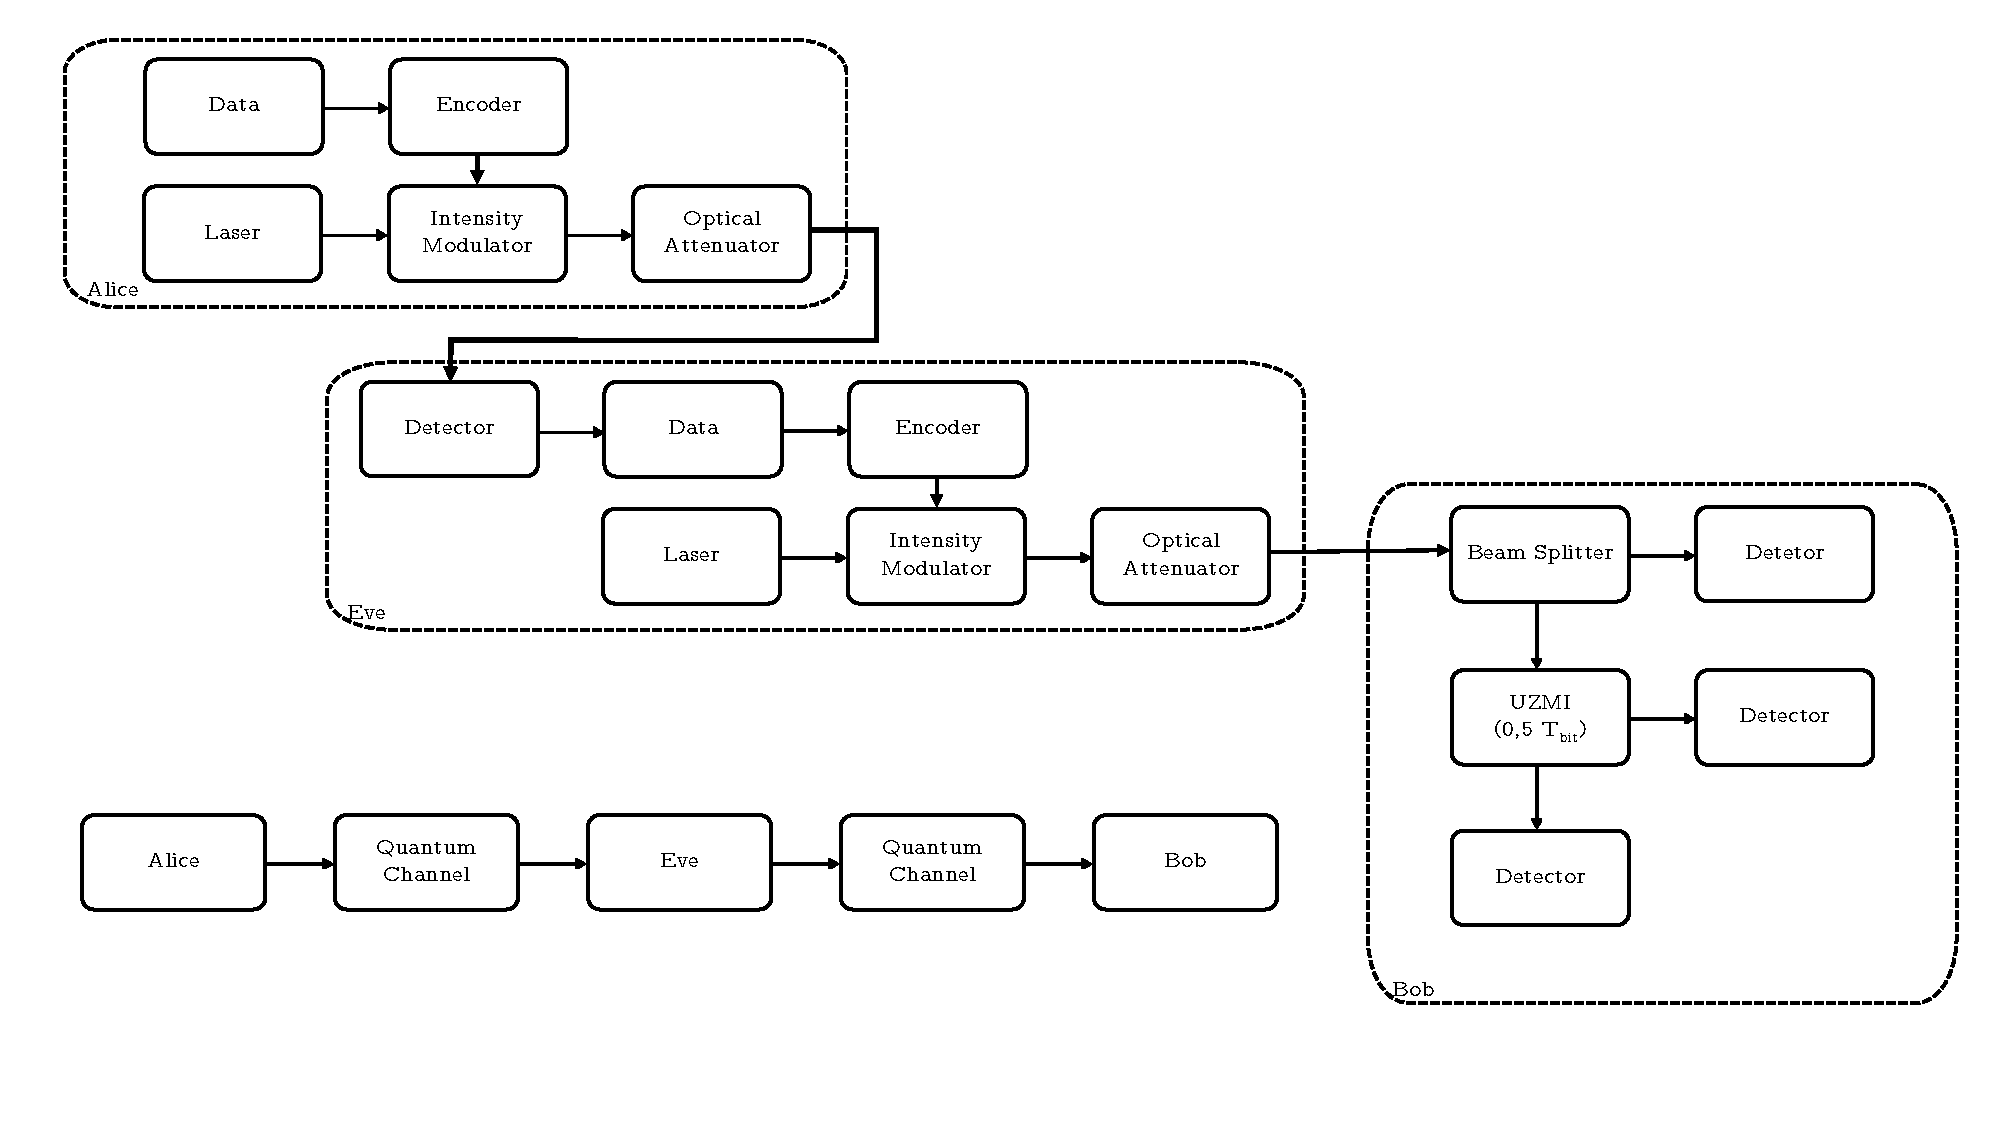
\includegraphics[width=1\linewidth]{./sdf/tq_76558_cow_protocol/slides/figures/Diagrama_de_blocos.pdf}
\caption{Block diagram for the basic IR attack.}
\label{fig:bloc}
\end{figure}

\begin{figure}[h]
\centering
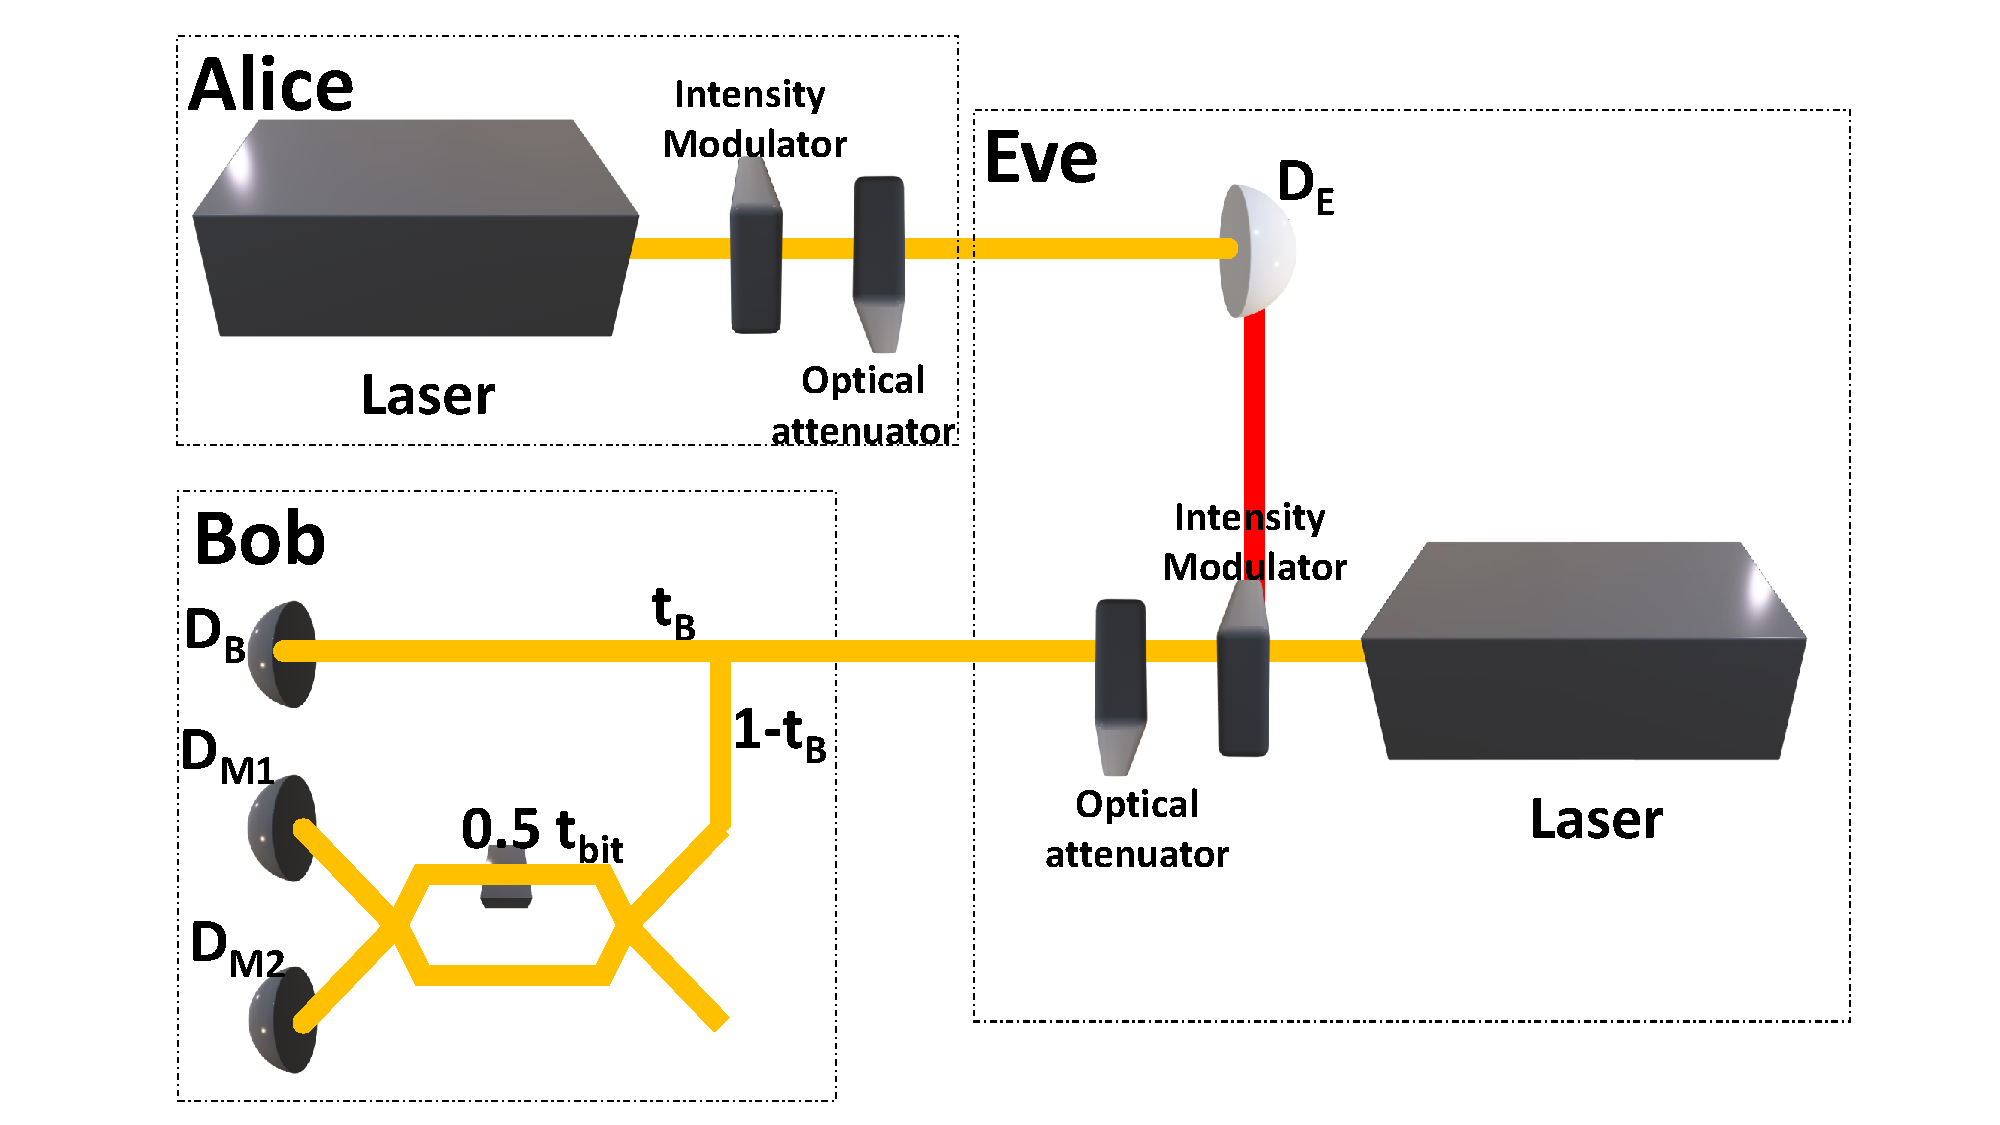
\includegraphics[width=1\linewidth]{./sdf/tq_76558_cow_protocol/slides/figures/E.pdf}
\caption{Simple scheme of the IR attack.}
\label{fig:E}
\end{figure}

As Eve as aces to the classic channel, she can remove the decoys times from her data line (step 4), and after in step five, she can delete all the times that Bob didn't had a click in his data line. So, in the End of step five she as the same key as Alice and Bob, they after calculating QBER, and she can also know in which bits will they calculate the QBER and delete also those bits from their data line. So, Eve as the complete key in the final of step sixth, and if she is not caught, she can later decrypt messages.

For the simulation, I created a function ``Alice'' that generates a string with $10^7$ characters, every one of this characters has a $10 \%$ chance of being a ``d'' - representing a decoy state ($|d\rangle$), and half of the rest ($45 \%$) of being a ``0'' and the same probability of being a ``1'' - representing a zero state ($|0\rangle$) and a one state ($|1\rangle$) correspondent. 

The output of this function is a string with size $2\times10^7$ where all the states, have been replaced by ``1'' and ``0'' corresponding to the photons state and the vacuum state, the states where created using a Poisson distribution, but the completely empty states were removed. So, this output variable has only the number of photons for every time bin, note that two-time bin is needed for any state.

In this ``Alice'' function the decoy state only has near 1\% of probability of having photons in both pulses, most of the decoy states will only have photon in one of the pulses (90 \%).

To generate this $10^7$ initial string, the protocol needs to be running for 0.1 if the fibber doesn't have loses, in Table \ref{Meaning} we can see how much of this $10^7$ characters get transformed into Logical bits for Bob in the end of stage 6. The following stage (7) would shorten even more the key.


\begin{table}[hbt!]
\centering
\scriptsize
\begin{tabular}{ccccccc}
$10^7$ & $\times 0.1$ & $\times 0.9$ & $\times 0.9$ & $\times 0.5$ & $\times 0.5$ & $=40 500$ \\
\begin{tabular}[c]{@{}c@{}}0.1 seconds\\ Alice raw\\ characters\end{tabular} & \begin{tabular}[c]{@{}c@{}}Average Nº\\ of photons by\\ impulse\end{tabular} & \begin{tabular}[c]{@{}c@{}}Bits that go \\ to the Data\\ line\end{tabular} & \begin{tabular}[c]{@{}c@{}}Logical bits\\ that are not \\ decoy states\end{tabular} & \begin{tabular}[c]{@{}c@{}}Used to \\ calculate\\ QBER\end{tabular} & \begin{tabular}[c]{@{}c@{}}Efficiency\\ of Bob's\\ Detectors\end{tabular} & \begin{tabular}[c]{@{}c@{}}Final bits in\\ in the end of\\ Stage 6\end{tabular}
\end{tabular}
\caption{How much key is produced in 0.1 seconds.}
\label{Meaning}
\end{table}

The second function called ``Eve'' captures all the information with her detector with a certain efficiency (the loses of the fibber were not simulated, wouldn't alter anything, would just make the simulation less efficient) and then using a Poisson distribution generates the photons that sends to Bob in the same time bins that she has measured. The output of this function is once again a string with size $2\times10^7$.

Finally, I have created a function called ``Bob'' that would measure the incoming photons in 3 detectors, all of them with the same efficiency, and with probability of dark counts. Any photon that enter as input can either go for the data line (10 \% of the photons), or for the monitoring line (90 \%), in the data line they are simply registered as they come, and only one photon is needed, more photons do not alter anything, if he doesn't receive any photon, it can still register due to dark counts. If the photon goes to monitoring line, then he goes to another beam splitter, this time with 50 \% probability for every outcome, in the first, he is delayed by half $time_{bin}$ (if he doesn't interact in the next unit of time fires the $D_{M1}$), on the other outcome he interacts with the delayed photon, if there is no delayed photon, he fires the $D_{M1}$, if there is he fires the $D_{M2}$.

For the final function ``QBER'', a simple function that removes the decoy times from the Bob and Eve, due to the information from Alice and calculates QBER using a percentage of the total information that Bob got in the data Line (50 \% in this simulation).

I have run the simulation 200 times and then studied the average (Mean), and the standard deviation (Std), the values that I've used as Inputs can be seen in Table \ref{Inputs}.

\subsection*{Inputs}

\begin{table}[hbt!]
\centering
\begin{tabular}{|c|c|}
\hline
Logical Bits from Alice & $10^{7} (0.1 s)$ \\ \hline
Probability of Decoy & 10 \% \\ \hline
Alice- Nº of Photons per pulse & 0.1\\ \hline
Bob Detectors Efficiency & 10 \% \\ \hline
Bob Dark Count Probability & $10^{-5}$ \\ \hline
Run over & $200 \times$\\ \hline
Percentage of the Key for QBER & 50 \% \\ \hline
\end{tabular}
\caption{Inputs used in the simulation.}
\label{Inputs}
\end{table}

\subsection*{Outputs}
This system outputs the following objects:

In a simulation without attack, using the variables seen in Table \ref{Inputs}, I obtain the results present in Table \ref{No IR}.

\begin{table}[hbt!]
\centering
\begin{tabular}{c|c|c|}
\cline{2-3}
& Mean & FFFFFF Std} \\ \hline
\multicolumn{1}{|c|}{QBER} & 1.366e-04 & 0.185e-04 \\ \hline
\multicolumn{1}{|c|}{ $D_B$}} & 423899 & 432.5 \\ \hline
\multicolumn{1}{|c|}{ $D_{M1}$}} & 96288.8 & 329.216 \\ \hline
\multicolumn{1}{|c|}{ $D_{M2}$}} & 59.615 & 8.531 \\ \hline
\end{tabular}
\caption{Results of a simulation without attack}
\label{No IR}
\end{table}

If I now analyse the IR attack using the average number of photons by impulse used by Eve equal to the same as used by Alice (modulated by a Poisson distribution with $\lambda=0.1$) and altering the values of her detector Efficiency. The results of this can be seen in Table \ref{IR1}

\begin{table}[hbt!]
\centering

\scriptsize
\begin{tabular}{c|c|c|c|c|c|c|c|c|}
\hline
\multicolumn{1}{|c|}{\begin{tabular}[c]{@{}c@{}}Eve\\ Efficiency\end{tabular}}} & \multicolumn{2}{c|}{10 \%}} & \multicolumn{2}{c|}{50 \%}} & \multicolumn{2}{c|}{{90 \%}} & \multicolumn{2}{c|}{{100 \%}} \\ \hline
 &{Mean} &{ Std} & { Mean} & { Std} & {Mean} &{Std} & {Mean} & {Std} \\ \hline
\multicolumn{1}{|c|}{ QBER}} & 0.800 & 0.363 & 0.223 & 0.367 & 0.012 & 0.060 & 24.0e-03 & 2.13e-03 \\ \hline
\multicolumn{1}{|c|}{ $D_B$}} & 3117 & 10274 & 21137 & 19737 & 36773 & 11334 & 40433 & 143 \\ \hline
\multicolumn{1}{|c|}{ $D_{M1}$}} & 683.4 & 2327.4 & 4788.8 & 4494.7 & 8340 & 2580 & 9166.3 & 99.1 \\ \hline
\multicolumn{1}{|c|}{ $D_{M2}$}} & 0.04 & 0.25 & 0.28 & 0.61 & 0.42 & 0.73 & 0.54 & 0.75 \\ \hline
\end{tabular}
\caption{Results of a simulation with attack changing the efficiency of Eve detector}
\label{IR1}
\end{table}

The second value that we can change for Eve is the average number of photons by impulse that she uses, of course this allows attacks of other Eves by beam splitters but supposing that she has a way of guarantying that no one else does attacks to the line. And, if she has a 100 \% efficiency or her detector (while Bob remains with the usual 10\%). The results of this case can be seen in Table \ref{IR2}.

\begin{table}[hbt!]
\centering
\begin{tabular}{ccccccc}
{\begin{tabular}[c]{@{}c@{}}Eve Avg. Num.\\  photons/Imp\end{tabular}} & \multicolumn{2}{c}{1.0001}} & \multicolumn{2}{c}{{1.1}} & \multicolumn{2}{c}{{1.2}} \\
 & { Mean} & { Std} & { Mean} & { Std} & { Mean} & { Std} \\
{ QBER} & 1.71e-03 & 0.15e-03 & 1.62e-03 & 0.20e-03 & 1.52e-03 & 0.17e-03 \\
{$D_B$} & 387664 & 665 & 424371 & 380.8 & 461107 & 569.7 \\
{$D_{M1}$} & 91434 & 232.5 & 100067 & 183.6 & 109942 & 614.0 \\
{$D_{M2}$} & 52 & 7.04 & 65.4 & 10.41 & 70.4 & 5.64
\end{tabular}
\caption{Results of a simulation with attack changing the average number of photons by impulse used by Eve}
\label{IR2}
\end{table}

\begin{table}[]
\begin{tabular}{ccccc}
{\begin{tabular}[c]{@{}c@{}}Eve Avg. Num.\\  photons/Imp\end{tabular}} & {\begin{tabular}[c]{@{}c@{}}No IR\\ Atack\end{tabular}} & {1.0001} & {1.1} & {1.2} \\
{$\frac{$B\_\{M1\}+B\_\{M2\}$}{Key Length}$} & 22.73 & 23.60 & 23.60 & 23.86
\end{tabular}
\caption{Results of a simulation with attack changing the average number of photons by impulse used by Eve analizing the results}
\label{IR3}
\end{table}

\pagebreak
\subsection{Conclusion - Simulation Results}

By having an efficiency lower than 100 \% Eve presence lowers the Key length ($D_B$) by one order of magnitude and increases the QBER.

And even if her efficiency is of 100 \%, Eve presence still increases the ratio $\frac{$B_{M1}+B_{M2}$}{Key Length}$ (now 24\%, without attack is 22\%), besides also increase the QBER by nearly one order of magnitude.

This allows us to see that the COW protocol is robust enough against a basic IR attack even in "paranoid" properties like her detectors having a 100\% efficiency and Dark Counts that is not very realistic while Bob's ones remain with 10 \% and with probabilities of Dark Counts.

% bibliographic references for the section ----------------------------
\clearpage
\printbibliography[heading=subbibliography]
\end{refsection}
\addcontentsline{toc}{subsection}{Bibliography}
\cleardoublepage
% --------------------------------------------------------------------- 
